
\subsubsection{ab KW50}
\begin{quote}
	\subsubsection*{Arbeit in der Schule}
	In meiner Git Repository konnte ich den Main Branch nicth finden. Anschließend habe ich folgende Befehle verwendet um das Problem zu lösen Abbildung: \ref{fig:screenshot02}.
	
	
	Charakter Direktorin erstellt
	Charakterskin und Animationen von Mixamo.com geholt
	Animation: einfaches ide zum stehen
	
	
	Meine nächste Aufgabe:
	Dialog mit Lehrer programmieren: Wenn Schüler in in der Nähe vom Lehrer oder Direktorin ist, soll ein Dialogfenster öffnen, wo das Gespräch läuft.
	Beim Dialog stellt der Lehrer nach einem kurzen Gespräch fragen an den Schüler.
	Schüler soll mit Buttons auf die Fragen antworten können.
	Wenn auf Fragen falsch beantwortet wird, soll sein leben weniger werden.
	
	Funktion:
	Wenn Schüler im Blickfeld(Triggerzone: Abbildung \ref{fig:triggerzone}) und die Taste F gedrückt wird soll das Dialogsystem das Dialogfenster öffnen.
	
	\subsubsection*{Arbeit außerhalb der Schule}
	
	Ich habe Wochenlang versucht, die Aufgabenstellung die ich beschrieben habe zu realisieren. Ich habe viele Programme gefunden, die sehr lange und komplex waren. Zum Schluss habe ich mich entschieden das Programm selber zu schreiben, welches sehr Zeit in Anspruch nahm.

	
	Übersicht Programm:
	
	1. Empty DialogueSystem: hier werden unsere Dialog GUIs sein, die mit dem Script DialogueSystem verwaltet werden. Diese entscheidet welches GUI geöffnet werden soll, indem Sie schaut ob das Gespräch eine Frage beinhaltet
	
	2. GUI DialogueUI: Hier werden die Gespräche im Textbox angezeigt
	
	3. DialogueUI Question Buttons: Dieses GUI wird angezeigt, wenn der Lehrer, dem Schüler eine Frage stellt. Somit kann also der Schüler mittels Buttons auf die Frage beantworten. Im Script DialogSystem werden die Antworten vom Spieler mit den richtigen Antworten vergleicht. Wenn die Antwort richtig ist wird der Button grün. Doch wenn die Antwort falsch wird der Button rot und das Leben vom Spieler wird weniger.
	
	Erledigte Aufgaben:
	
	4. Die schon davor programmierte, statische Gegner ins Spiel platziert
	
	5. Dynamischer Gegner programmiert : Abbildung \ref{fig:dynamischergegner}
	
	Funktion:
	
		Wenn Hauptcharakter im Blickfeld: Leben wird reduziert
		
		Figur bewegt sich zwischen den angegebenen Koordinaten
		
	Programm Übersicht:
	
	NavMesh Agent Component: Figur bewegen
	
	Parameter(Zielkoordinaten als Array, Figur)
	
	Programmstart: Figur geht zur Zielkoordinate[0]
	
	Wenn die Figur ihr Ziel erreicht hat: nächstes Ziel
	
	6. Es wurde ein Healthbar(Lebensskala) programmiert. Wenn der Hauptcharakter in Sicht eines Gegners kommt wird sein Leben weniger.
	
	Veränderungen an statischen und dynamischen Gegnern vorgenommen: Healthbar Funktion eingefügt und Werte angepasst
	
	7. Andere Charakter Lehrpersonen aus der Website Maximo.com geholt und sie entsprechend angepasst. Abbildung: \ref{fig:anderecharakter}
	
	8. Semih Can beim Multiplayerprogramm weitergeholfen
	
	\begin{figure}
		\centering
		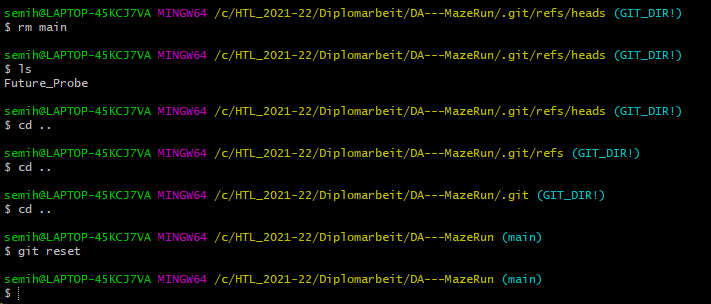
\includegraphics[width=0.7\linewidth]{img/SemihSoenmez_IMG/screenshot02}
		\caption{}
		\label{fig:screenshot02}
	\end{figure}
	\begin{figure}
		\centering
		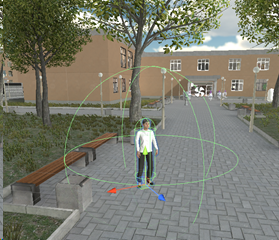
\includegraphics[width=0.3\linewidth]{img/SemihSoenmez_IMG/Triggerzone}
		\caption{}
		\label{fig:triggerzone}
	\end{figure}

	\begin{figure}
		\centering
		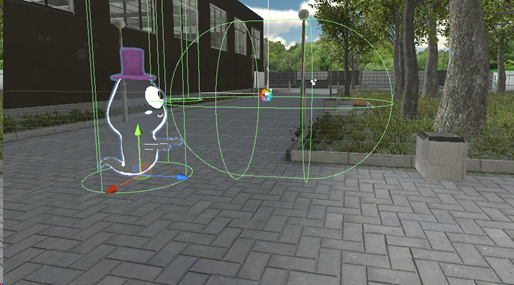
\includegraphics[width=0.5\linewidth]{img/SemihSoenmez_IMG/dynamischerGegner}
		\caption{}
		\label{fig:dynamischergegner}
	\end{figure}

	\begin{figure}
		\centering
		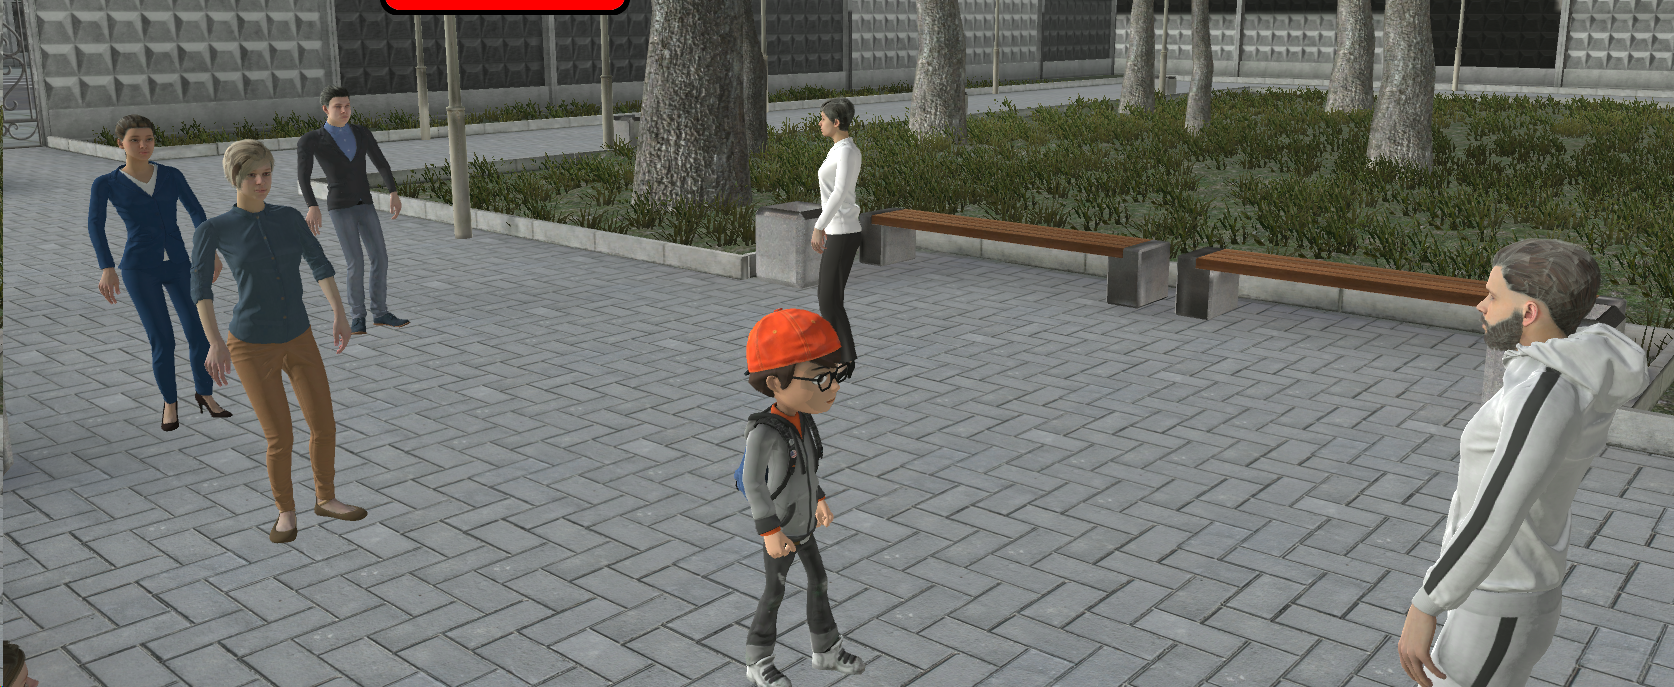
\includegraphics[width=0.7\linewidth]{img/SemihSoenmez_IMG/andereCharakter}
		\caption{}
		\label{fig:anderecharakter}
	\end{figure}


	

	


\end{quote}
